% Template for PLoS

\documentclass[10pt]{article}
\usepackage[utf8]{inputenc}

% amsmath package, useful for mathematical formulas
\usepackage{amsmath}
% amssymb package, useful for mathematical symbols
\usepackage{amssymb}

% hyperref package, useful for hyperlinks
\usepackage{hyperref}

% graphicx package, useful for including eps and pdf graphics
% include graphics with the command \includegraphics
\usepackage{graphicx}

% Sweave(-like)
\usepackage{fancyvrb}
\DefineVerbatimEnvironment{Sinput}{Verbatim}{fontshape=sl}
\DefineVerbatimEnvironment{Soutput}{Verbatim}{}
\DefineVerbatimEnvironment{Scode}{Verbatim}{fontshape=sl}
\newenvironment{Schunk}{}{}
\DefineVerbatimEnvironment{Code}{Verbatim}{}
\DefineVerbatimEnvironment{CodeInput}{Verbatim}{fontshape=sl}
\DefineVerbatimEnvironment{CodeOutput}{Verbatim}{}
\newenvironment{CodeChunk}{}{}

% cite package, to clean up citations in the main text. Do not remove.
\usepackage{cite}

\usepackage{color}

% Use doublespacing - comment out for single spacing
%\usepackage{setspace}
%\doublespacing


% Text layout
\topmargin 0.0cm
\oddsidemargin 0.5cm
\evensidemargin 0.5cm
\textwidth 16cm
\textheight 21cm

% Bold the 'Figure #' in the caption and separate it with a period
% Captions will be left justified
\usepackage[labelfont=bf,labelsep=period,justification=raggedright]{caption}

% Use the PLoS provided bibtex style
\bibliographystyle{plos}

% Remove brackets from numbering in List of References
\makeatletter
\renewcommand{\@biblabel}[1]{\quad#1.}
\makeatother


% Leave date blank
\date{}

\pagestyle{myheadings}
%% ** EDIT HERE **


%% ** EDIT HERE **
%% PLEASE INCLUDE ALL MACROS BELOW

%% END MACROS SECTION


\begin{document}

% Title must be 150 characters or less
\begin{flushleft}
{\Large
\textbf{A Capitalized Title: Something about a great Discovery}
}
% Insert Author names, affiliations and corresponding author email.
\\
  FirstName LastName\textsuperscript{1,2*},
  Second Author\textsuperscript{3}\\
\bf{1} Dept/Program/Center, Institution Name,  City,  State,  Country
\\
\bf{2} Dept/Program/Center, Institution Name,  City,  State,  Country
\\
\bf{3} Dept/Program/Center, Institution Name,  City,  State,  Country
\\
\bf{4} Dept/Program/Center, Institution Name,  City,  State,  Country
\\

\textasteriskcentered{} E-mail:   \href{mailto:name@company.com}{\nolinkurl{name@company.com}}


\end{flushleft}

\section*{Abstract}\label{abstract}
\addcontentsline{toc}{section}{Abstract}

Please keep the abstract between 250 and 300 words

\section*{Author summary}\label{author-summary}
\addcontentsline{toc}{section}{Author summary}

Please keep the Author Summary between 150 and 200 words Use first
person. PLoS ONE authors please skip this step. Author Summary not valid
for PLoS ONE submissions.

\section*{Introduction}\label{introduction}
\addcontentsline{toc}{section}{Introduction}

Cite fancy references (Garnier et al., 2007).

\section*{Results}\label{results}
\addcontentsline{toc}{section}{Results}

Results and Discussion can be combined.

\subsection*{Subsection 1}\label{subsection-1}
\addcontentsline{toc}{subsection}{Subsection 1}

You can use R chunks directly to plot graphs.

\begin{CodeChunk}
\begin{CodeInput}
require("ggplot2")
x <- 0:100
y <- 2 * (x + rnorm(length(x), sd = 3) + 3)
ggplot(data = data.frame(x, y),
       aes(x = x, y = y)) +
  geom_point() +
  geom_smooth(method = "lm")
\end{CodeInput}
\begin{figure}

{\centering 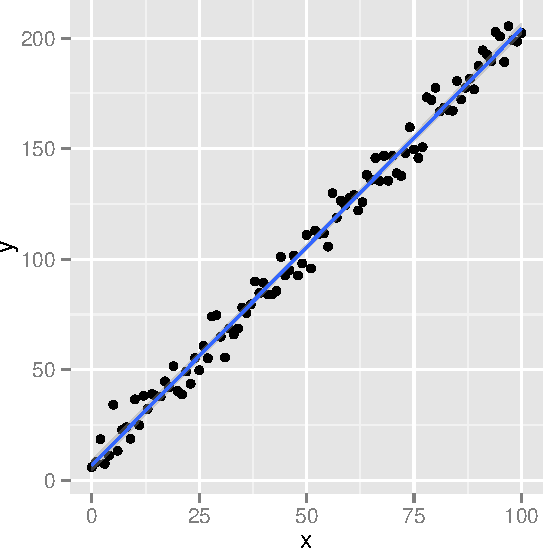
\includegraphics{skeleton_files/figure-latex/graph-1}

}

\caption[Figure caption]{Figure caption}\label{fig:graph}
\end{figure}
\end{CodeChunk}

\subsection*{Subsection 2}\label{subsection-2}
\addcontentsline{toc}{subsection}{Subsection 2}

\section*{Discussion}\label{discussion}
\addcontentsline{toc}{section}{Discussion}

\section*{Material and Methods}\label{material-and-methods}
\addcontentsline{toc}{section}{Material and Methods}

You may title this section ``Methods'' or ``Models''. ``Models'' is not
a valid title for PLoS ONE authors. However, PLoS ONE authors may use
``Analysis''

\section*{Acknowledgments}\label{acknowledgments}
\addcontentsline{toc}{section}{Acknowledgments}

Do NOT remove this, even if you are not including acknowledgments

\section*{References}\label{references}
\addcontentsline{toc}{section}{References}

A reference list should be automatically created here. However it won't.
Pandoc will place the list of references at the end of the document
instead. There are no convenient solution for now to force Pandoc to do
otherwise. The easiest way to get around this problem is to edit the
LaTeX file created by Pandoc before compiling it again using the
traditional LaTeX commands.

\section*{Figure Legends}\label{figure-legends}
\addcontentsline{toc}{section}{Figure Legends}

\section*{Tables}\label{tables}
\addcontentsline{toc}{section}{Tables}

Garnier, S., Gautrais, J., Theraulaz, G., 2007. The biological
principles of swarm intelligence. Swarm Intelligence 1, 3--31.
doi:\href{http://dx.doi.org/10.1007/s11721-007-0004-y}{10.1007/s11721-007-0004-y}

\end{document}

